\documentclass[../../deep_learning_notes.tex]{subfiles}
\begin{document}
%%%%%%%%%%%%%%%%%%%%%%%%%%%%%%
\section{Backpropagation Example}
We consider the following network for classification ($N$ is the batch size)
\begin{alignat*}{2}
    X_{1} &= XW_{1} + b_{1} \quad &X \in \mathbb{R}^{2}, W_{1} \in \mathbb{R}^{2 \times 4}, b_{1} \in \mathbb{R}^{4}\\
    X_{1r} &= ReLU(X_{1})\\
    X_{2} &= X_{1r}W_{2} + b_{2} \quad &W_{2} \in \mathbb{R}^{4 \times 2}, b_{2} \in \mathbb{R}^{2}\\
    X_{2r} &= ReLU(X_{2})\\
    X_{3} &= X_{2r}W_{3} + b_{3} \quad &W_{3} \in \mathbb{R}^{2 \times 1}, b_{3} \in \mathbb{R}\\
    \hat{y} &= \sigma(X_{3})\\
    L &= -\frac{1}{N} \bigg( y^{T}log(\hat{y}) + (1 - y)^{T}log(1 - \hat{y}) \bigg)
\end{alignat*}

Based on the previous derivations, we work backwards to calculate gradients
\begin{alignat*}{2}
    \frac{dL}{d\hat{y}} & & &= -\frac{1}{N} \bigg( \frac{y}{\hat{y}} - \frac{1-y}{1-\hat{y}} \bigg)\\
    \frac{dL}{dX_{3}} &= \frac{dL}{d\hat{y}} \frac{d\hat{y}}{dX_{3}}
    & &= \frac{dL}{d\hat{y}} \odot \sigma(X_{3}) \odot (1 - \sigma(X_{3}))\\
    \frac{dL}{dW_{3}} &= \frac{dL}{dX_{3}} \frac{dX_{3}}{dW_{3}} & &= X_{2r}^{T} \frac{dL}{dX_{3}}\\
    \frac{dL}{db_{3}} &= \frac{dL}{dX_{3}} \frac{dX_{3}}{db_{3}} & &= \bm{1}_{N}^{T}\frac{dL}{dX_{3}}\\
    \frac{dL}{dX_{2r}} &= \frac{dL}{dX_{3}} \frac{dX_{3}}{dX_{2r}} & &= \frac{dL}{dX_{3}}W_{3}^{T}\\
\end{alignat*}
\begin{alignat*}{2}
    \frac{dL}{dX_{2}} &= \frac{dL}{dX_{2r}} \frac{dX_{2r}}{dX_{2}} & &=\frac{dL}{dX_{2r}} \odot (X_{2} > 0)\\
    \frac{dL}{dW_{2}} &= \frac{dL}{dX_{2}} \frac{dX_{2}}{dW_{2}} & &= X_{1r}^{T} \frac{dL}{dX_{2}}\\
    \frac{dL}{db_{2}} &= \frac{dL}{dX_{2}} \frac{dX_{2}}{db_{2}} & &= \bm{1}_{N}^{T} \frac{dL}{dX_{2}}\\
    \frac{dL}{dX_{1r}} &= \frac{dL}{dX_{2}} \frac{dX_{2}}{dX_{1r}} & &=\frac{dL}{dX_{2}} W_{2}^{T}\\
\end{alignat*}
\begin{alignat*}{2}
    \frac{dL}{dX_{1}} &= \frac{dL}{dX_{1r}} \frac{dX_{1r}}{dX_{1}} & &= \frac{dL}{dX_{1r}} \odot (X_{1} > 0)\\
    \frac{dL}{dW_{1}} &= \frac{dL}{dX_{1}} \frac{dX_{1}}{dW_{1}} & &= X^{T}\frac{dL}{dX_{1}}\\
    \frac{dL}{db_{1}} &= \frac{dL}{dX_{1}} \frac{dX_{1}}{db_{1}} & &= \bm{1}_{N}^{T}\frac{dL}{dX_{1}}\\
\end{alignat*}
Figure \ref{fig:gradient_backprop_example_1} shows how the final output looks on some sample data (with noise). The two classes are separated by a non-linear circular boundary.

\begin{figure}[h]
    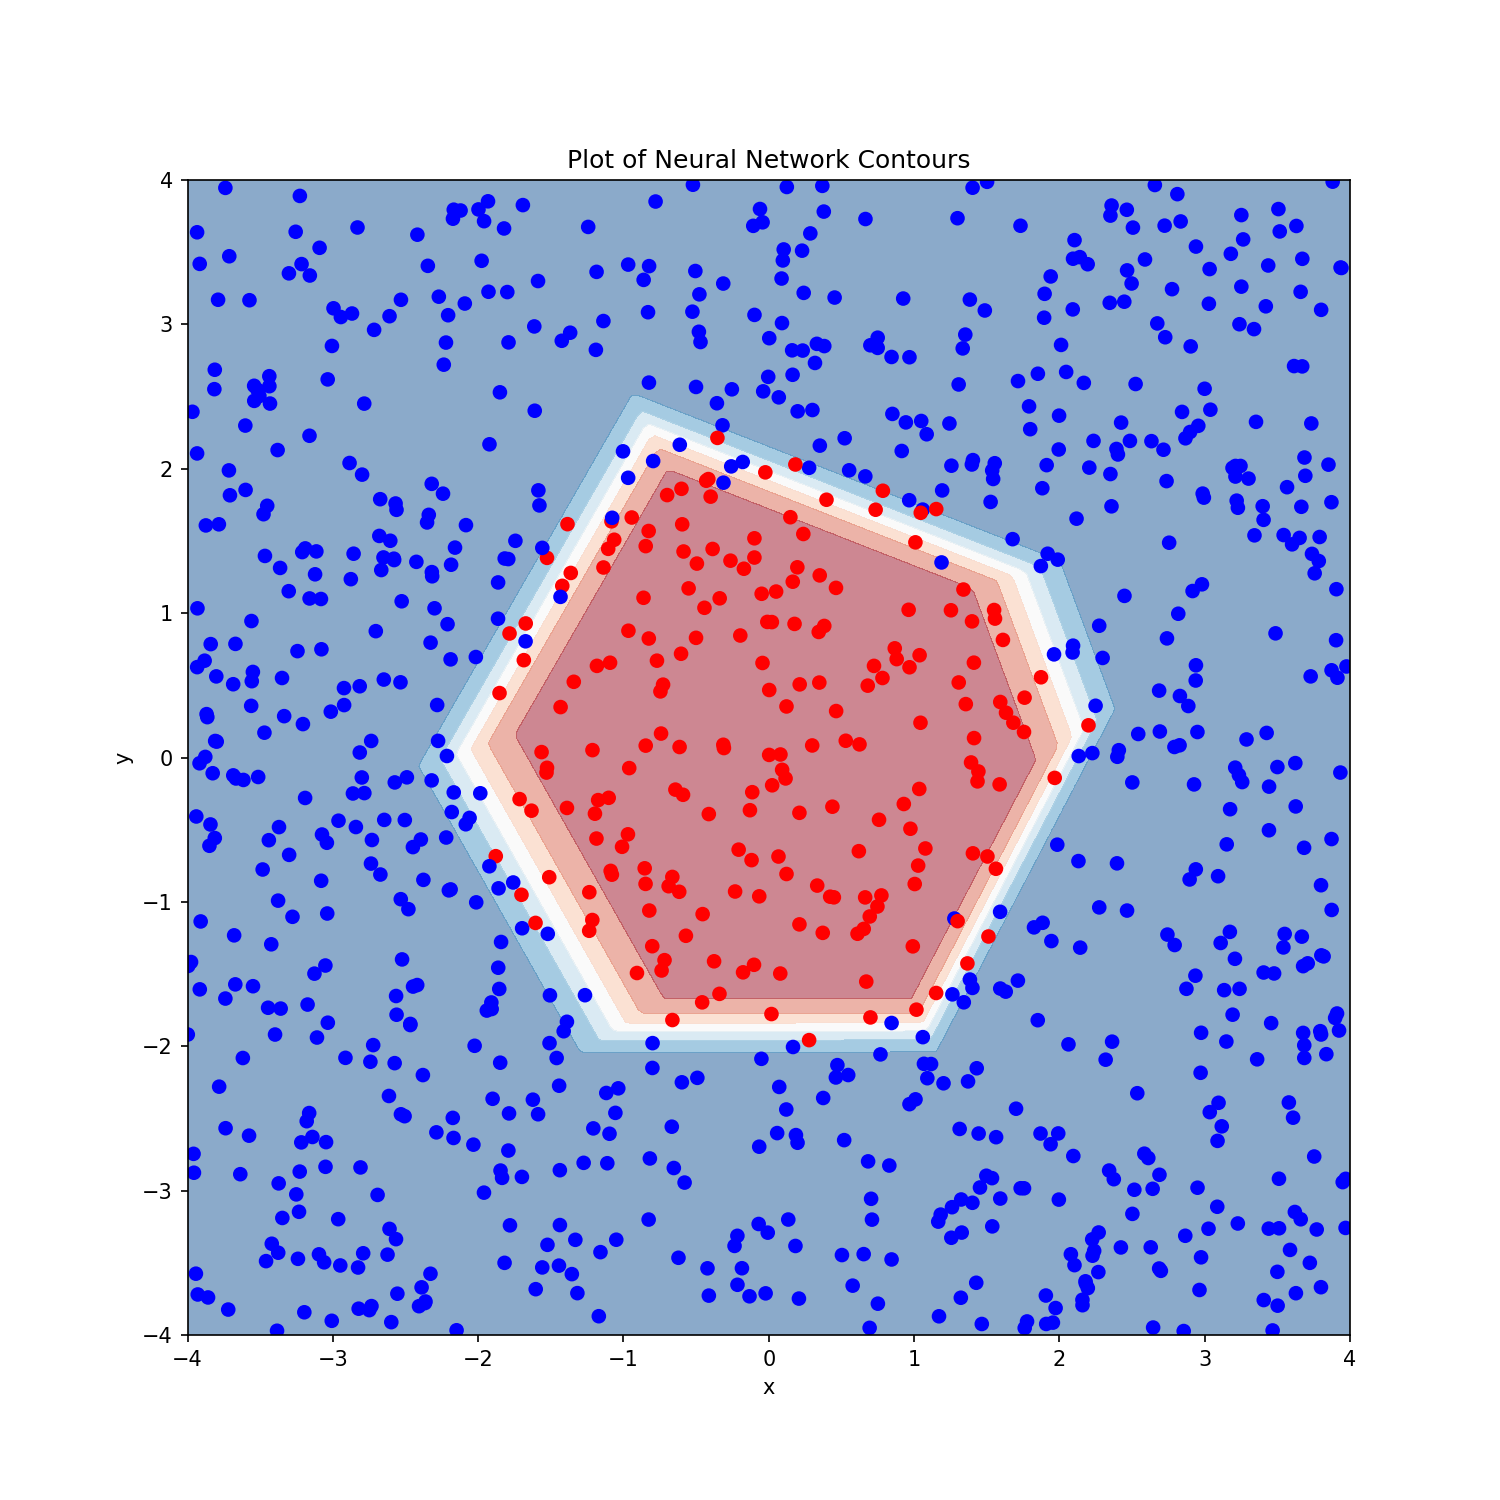
\includegraphics[scale=0.4]{gradient_backprop_example_1}
    \centering
    \caption {Red and Blue points represent two classes. The coloured countours represent the final predictions of the neural network on the entire surface. Plot prepared using backprop\_example\_1.py.}
    \label{fig:gradient_backprop_example_1} %\ref{fig:gradient_backprop_example_1}
\end{figure}
\end{document}